% !TeX program = xelatex
\documentclass[aspectratio=169,11pt]{beamer}

\usepackage{graphicx}
\usepackage{booktabs}
\usepackage{array}
\usepackage{tikz}
\usetikzlibrary{positioning,arrows.meta,calc,shadows}
\usepackage{fontawesome5}
\usepackage{hyperref}
\usepackage{amsmath}
\usepackage{natbib}

\usepackage{theme/beamerthemeResearch}

\title[Decision Assistance \& Steering]{Decision Assistance and Steering\\ in Health Insurance}
\subtitle{Brown bag}
\author{%
  \begin{tabular}[t]{@{}l@{\hspace{1.5cm}}l@{}}
    Ian McCarthy & Evan Saltzman \\[2pt]
    {\usebeamerfont{institute}\usebeamercolor[fg]{institute}Emory University} &
    {\usebeamerfont{institute}\usebeamercolor[fg]{institute}Florida State University}
  \end{tabular}}
\institute{}
\date{October 15, 2026}

% ── Reusable stat callout: \statbox{width}{big number}{caption} ──
\newcommand{\statbox}[3]{%
  \begin{minipage}[t]{#1}
    \centering
    {\Huge\bfseries\color{emoryBlue}#2}\\[0.15cm]
    {\small\color{emoryDark}#3}
  \end{minipage}%
}

% ── Clickable "Help!" popup (adapted from the AHEW discussion deck) ──
% The frame is shown as overlay <1> in the talk, with a "Help!" button in the
% top-right corner. Clicking it jumps to overlay <2>, a copy of the slide dimmed
% behind a card describing where we would like input, typeset after the appendix
% by \againframe. The card's close button jumps back to <1>; pressing next from <1>
% skips the card.
%   Usage: \begin{frame}<1>[label=help-x]{Title} ... \helpcard{help-x}{Text.} \end{frame}
%          and, at the end of the document, \againframe<2>{help-x}
%   On a frame that steps through n clicks, show <1-n>, call
%   \helpcard[n+1][n]{help-x}{Text.}, and use \againframe<n+1>{help-x}.
%   \helpcard must be the last thing in the frame so the card is drawn on top.
\NewDocumentCommand{\helpcard}{O{2} O{1} m +m}{%
  \alt<#1>{%
  \setcounter{framenumber}{\csname helpnum#3\endcsname}%
  \helpcardbody{#3<#2>}{#4}}{%
  \expandafter\xdef\csname helpnum#3\endcsname{\arabic{framenumber}}%
  \begin{tikzpicture}[remember picture, overlay]
    \node[anchor=east, fill=emoryBlue, text=white, font=\scriptsize\bfseries,
          rounded corners=7pt, inner sep=0pt]
      at ([xshift=-1.5cm, yshift=0.33cm]current page.south east)
      {\hyperlink{#3<#1>}{\rule[-5pt]{0pt}{16pt}\hspace{9pt}Help!\hspace{9pt}}};
  \end{tikzpicture}}%
}
\newcommand{\helpcardbody}[2]{%
  \begin{tikzpicture}[remember picture, overlay]
    \fill[white, opacity=0.78] (current page.south west) rectangle (current page.north east);
    \node[fill=white, rounded corners=6pt, drop shadow={opacity=0.30, shadow xshift=2pt, shadow yshift=-2pt},
          inner xsep=18pt, inner ysep=16pt]
      (card) at ([yshift=-0.2cm]current page.center)
      {\parbox{11.6cm}{\normalsize\color{emoryDark}\raggedright\hyphenpenalty=10000 \exhyphenpenalty=10000
       #2\par}};
    \fill[emoryBlue] ([xshift=7pt, yshift=-12pt]card.north west) rectangle ([xshift=10pt, yshift=12pt]card.south west);
    \node[circle, fill=emoryBlue, text=white, font=\scriptsize\bfseries, inner sep=0pt,
          minimum size=0.5cm] at (card.north east)
      {\hyperlink{#1}{\makebox[0.5cm]{\rule[-4pt]{0pt}{14pt}$\times$}}};
  \end{tikzpicture}%
}

% ── Newspaper-clipping text pieces for the intermediaries slide ──
\newcommand{\clipheadline}[1]{{\rmfamily\bfseries #1}}
\newcommand{\clipsource}[1]{{\tiny\color{emoryMid}#1}}

\begin{document}

% Title
\begin{frame}[plain,noframenumbering]
  \titlepage
\end{frame}

% ── Motivation ──────────────────────────────────────────────
\section{Motivation}
\sectionframe

\begin{frame}[t]{Intermediaries common in complex purchases}
  \begin{center}
  \begin{tikzpicture}[
    bigicon/.style={text=emoryBlue,font=\fontsize{52}{52}\selectfont},
    dock/.style={align=center,font=\small,text=emoryDark},
    dockicon/.style={text=emoryBlue,font=\fontsize{22}{22}\selectfont},
    clip/.style={fill=white,draw=emoryRule,drop shadow={opacity=0.25},
      text width=7.4cm,align=left,inner sep=9pt,text=emoryDark,font=\small,
      execute at begin node={\raggedright\hyphenpenalty=10000 \exhyphenpenalty=10000 }},
  ]
    % Bounding box covers only the docked row, so the cards below can be drawn
    % over the space the bullets occupy later without moving anything
    \useasboundingbox (-0.2,-1.0) rectangle (13.2,1.1);

    % Docked row (appears once each card has had its turn)
    \node<2->[dockicon] at (2.2,0.65) {\faHome};
    \node<2->[dock] at (2.2,-0.3) {Home buyers\\{\scriptsize\color{emoryMid}realtors}};
    \node<3->[dockicon] at (6.5,0.65) {\faMoneyBillWave};
    \node<3->[dock] at (6.5,-0.3) {Investors\\{\scriptsize\color{emoryMid}financial advisers}};
    \node<4->[dockicon] at (10.8,0.65) {\faBriefcaseMedical};
    \node<4->[dock] at (10.8,-0.3) {Insurance buyers\\{\scriptsize\color{emoryMid}agents}};

    % Card 1: realtors
    \node<1>[bigicon] at (2.2,-2.55) {\faHome};
    \node<1>[clip,rotate=1.5] at (8.4,-2.55) {%
      \clipheadline{88\% of home buyers purchased through an agent or broker}\\[4pt]
      NAR paid \$418 million to settle home sellers' claims over broker commissions; offers of buyer-broker compensation can no longer be posted on the MLS.\\[4pt]
      \clipsource{NAR 2025 Profile of Home Buyers and Sellers; NAR settlement, approved Nov.\ 2024}};

    % Card 2: financial advisers
    \node<2>[bigicon] at (2.2,-2.55) {\faMoneyBillWave};
    \node<2>[clip,rotate=-1.2] at (8.4,-2.55) {%
      \clipheadline{7\% of financial advisers have misconduct records}\\[4pt]
      More than 15\% at some of the largest firms. About half lose their job after misconduct, and the labor market partially undoes that discipline by rehiring them.\\[4pt]
      \clipsource{Egan, Matvos, and Seru, \emph{Journal of Political Economy} 2019}};

    % Card 3: insurance agents
    \node<3>[bigicon] at (2.2,-2.55) {\faBriefcaseMedical};
    \node<3>[clip,rotate=1] at (8.4,-2.55) {%
      \clipheadline{43.7\% of new Medicare Advantage enrollees used an agent in 2022}\\[4pt]
      \$10.1 billion in agent commissions that year. In the ACA exchanges, 78\% of active enrollments were agent-facilitated in 2024.\\[4pt]
      \clipsource{Meyers et al., \emph{JAMA Internal Medicine} 2026; G\"urel, \emph{Risk Management and Insurance Review} 2024}};
  \end{tikzpicture}
  \end{center}

  \begin{itemize}
    \item<4-> Intermediaries help consumers understand the product and complete the purchase
    \item<5-> \emph{but} intermediaries are also paid commissions, introducing potential steering incentives and potentially inflating costs for all consumers
  \end{itemize}

  \vspace{0.2cm}
  \onslide<6->{\textbf{Questions:} How much do intermediaries steer customers versus improve choices? What are the implications for consumer welfare? And would we be better off with a more regulated commission environment?}
\end{frame}

\begin{frame}{Covered California offers commissioned and uncommissioned assistance side by side}
  \begin{center}
  {\scriptsize\color{emoryMid} Share of Covered California enrollments, 2014--2019.}    
  \begin{tikzpicture}[x=12cm,y=1cm,
    lab/.style={anchor=north,align=center,font=\small,text=emoryDark},
    pct/.style={font=\large\bfseries}]
    % segment widths are the channel shares in results/tables/assistance_channels.tex
    \useasboundingbox (0,-1.1) rectangle (1,1.3);
    \fill<1->[emoryGold] (0,0)     rectangle (0.452,1.3);
    \fill<2->[emoryBlue] (0.452,0) rectangle (0.640,1.3);
    \fill<3->[emoryRule] (0.640,0) rectangle (1,1.3);
    \node<1->[pct,text=white]     at (0.226,0.65) {45\%};
    \node<2->[pct,text=white]     at (0.546,0.65) {19\%};
    \node<3->[pct,text=emoryDark] at (0.820,0.65) {36\%};
    \node<1->[lab] at (0.226,-0.1) {Private agent\\{\scriptsize\color{emoryMid}paid a commission by the insurer}};
    \node<2->[lab] at (0.546,-0.1) {Public navigator\\{\scriptsize\color{emoryMid}no plan-specific pay}};
    \node<3->[lab] at (0.820,-0.1) {No assistance};
  \end{tikzpicture}
  \end{center}

  \vspace{0.3cm}
  \begin{itemize}
    \item<4-> Setting with lots of households making complex choices
    \item<5-> Mix of choices with commissioned help, uncommissioned help, and no help in the same market
  \end{itemize}
\end{frame}

\begin{frame}{What we do}
  Consumer-level enrollment data from the California ACA exchange, 2014--2019.

  \vspace{0.2cm}
  \begin{enumerate}
    \item<1-> Design-based estimate of how decision assistance affects plan choice (silver plan and dominated-plan selection)
    \item<2-> Structural model of household choice + insurer pricing and commissions
    \item<3-> Counterfactuals: remove assistance, defund navigators, reshape commissions, ban commissions
  \end{enumerate}
\end{frame}

% ── Data and Setting ────────────────────────────────────────
\section{Data and Setting}
\sectionframe

\begin{frame}[t]{Covered California is the state's ACA marketplace}
  \vspace{0.2cm}
  Roughly one million enrolled households a year after 2014, buying from 10--12 insurers.

  \vspace{0.4cm}
  \begin{columns}[t,onlytextwidth]
    \column{0.47\textwidth}
      \onslide<2->{%
      {\bfseries\color{emoryBlue} Plans}
      \begin{itemize}
        \item Four metal tiers: bronze, silver, gold, platinum
        \item Cost sharing standardized within a tier; plans differ by insurer, network, and premium
        \item 19 rating regions; choice sets (mainly) by region
        \item Premiums vary only by age (up to 3:1) and rating region
      \end{itemize}}
    \column{0.47\textwidth}
      \onslide<3->{%
      {\bfseries\color{emoryBlue} Subsidies}
      \begin{itemize}
        \item Premium subsidies up to 400\% FPL, tied to the second-cheapest silver plan; about 90\% of enrollees eligible
        \item Cost-sharing reductions below 250\% FPL, available only in silver plans
      \end{itemize}}
  \end{columns}
\end{frame}

\begin{frame}[t]{Agents are paid by insurers; navigators are not}
  \vspace{0.3cm}
  \begin{columns}[t,onlytextwidth]
    \column{0.47\textwidth}
      {\bfseries\color{emoryGold} Agents and brokers}
      \begin{itemize}
        \item Licensed, and certified by Covered California
        \item Paid a commission by the insurer, either a flat amount per member or a percent of premium
        \item About \$160 per member per year on average, paid each year the household stays enrolled
        \item Rates vary across insurers and are stable within an insurer
      \end{itemize}
    \column{0.47\textwidth}
      \onslide<2->{%
      {\bfseries\color{emoryBlue} Navigators}
      \begin{itemize}
        \item Enrollment counselors and service-center staff
        \item Funded by the exchange through an assessment on premiums
        \item No pay tied to the plan a household chooses
        \item Tend to work with lower-income, uninsured, and non-native English-speaking households
      \end{itemize}}
  \end{columns}
\end{frame}

\begin{frame}[t]{The data cover every Covered California enrollment, 2014--2019}
  \vspace{0.2cm}
  \begin{columns}[t,onlytextwidth]
    \column{0.50\textwidth}
      \begin{itemize}
        \item Enrollment records: plan, age, income, region, and assistance channel
        \item Uninsured years from each household's own years off the exchange
        \item Plan menus, premiums, commission schedules, and rate filings
        \item Nearly 8 million household-years
      \end{itemize}
    \column{0.45\textwidth}
      \onslide<2->{%
      \centering
      {\small\bfseries Enrolled household-years}\\[0.2cm]
      \footnotesize
      \begin{tabular}{lrr}
        \toprule
         & Assisted & Unassisted \\
        \midrule
        Household-years & 3.48M & 1.92M \\
        Income ($\times$ FPL) & 2.22 & 2.38 \\
        Age 18--34 & 26\% & 37\% \\
        Age 55--64 & 33\% & 24\% \\
        \bottomrule
      \end{tabular}\\[0.2cm]
      {\scriptsize\color{emoryMid} Assisted households are older and somewhat lower income.}}
  \end{columns}
\end{frame}

% ── Decision Assistance and Plan Choice ─────────────────────
\section{Does Assistance Improve Choices?}
\sectionframe

\begin{frame}{Design: predict the unassisted choice, compare to the assisted one}
  Inverse-propensity-weighted conditional logit estimated on unassisted households.

  \vspace{0.3cm}
  Use it to predict what assisted households would have chosen absent assistance -- an ATT on the treated.
\end{frame}

\begin{frame}{Cost-sharing reductions make gold and platinum dominated choices at low incomes}
  \begin{center}
  \begin{tikzpicture}[x=26cm,y=1cm,
    tier/.style={circle,minimum size=9pt,inner sep=0pt},
    tlab/.style={anchor=south,font=\small,text=emoryDark},
    vlab/.style={anchor=north,font=\scriptsize,text=emoryMid}]
    % actuarial values from results/tables/cost_sharing_schedule.tex
    \useasboundingbox (0.50,-1.5) rectangle (0.985,1.3);
    \draw[emoryRule,very thick] (0.57,0) -- (0.97,0);
    \node[anchor=east,font=\scriptsize,text=emoryMid,align=right] at (0.565,0) {Actuarial\\value};
    \foreach \av/\name in {0.60/Bronze, 0.80/Gold, 0.90/Platinum} {
      \node[tier,fill=emoryMid] at (\av,0) {};
      \node[tlab] at (\av,0.2) {\name};
      \node[vlab] at (\av,-0.2) {\av};
    }
    % silver moves up the axis as income falls
    \node<1>[tier,fill=emoryBlue] at (0.70,0) {};
    \node<1>[tlab,text=emoryBlue,font=\small\bfseries] at (0.70,0.2) {Silver};
    \node<1>[vlab] at (0.70,-0.2) {0.70};
    \node<2->[tier,draw=emoryBlue,fill=white] at (0.70,0) {};
    \node<2->[vlab] at (0.70,-0.2) {0.70};
    \node<2>[tier,fill=emoryBlue] at (0.87,0) {};
    \node<2>[tlab,text=emoryBlue,font=\small\bfseries,align=center] at (0.87,0.55) {Silver\\[-2pt]{\scriptsize 150--200\% FPL}};
    \node<2>[vlab] at (0.87,-0.2) {0.87};
    \node<3->[tier,fill=emoryBlue] at (0.94,0) {};
    \node<3->[tlab,text=emoryBlue,font=\small\bfseries,align=center] at (0.94,0.55) {Silver\\[-2pt]{\scriptsize 100--150\% FPL}};
    \node<3->[vlab] at (0.94,-0.2) {0.94};
    \draw<2>[-{Stealth},emoryBlue,thick] (0.71,-0.6) to[bend right=20] (0.86,-0.6);
    \draw<3->[-{Stealth},emoryBlue,thick] (0.71,-0.6) to[bend right=20] (0.93,-0.6);
  \end{tikzpicture}
  \end{center}

  \begin{itemize}
    \item<2-> 150--200\% FPL: silver is more generous and cheaper than gold
    \item<3-> 100--150\% FPL: silver is more generous and cheaper than gold and platinum
    \item<4-> Choosing a dominated plan is a mistake without needing a model of preferences
  \end{itemize}
\end{frame}

\begin{frame}{Assistance cuts dominated-plan selection by 42\%}
  \begin{columns}[c,onlytextwidth]
    \column{0.55\textwidth}
      \centering
      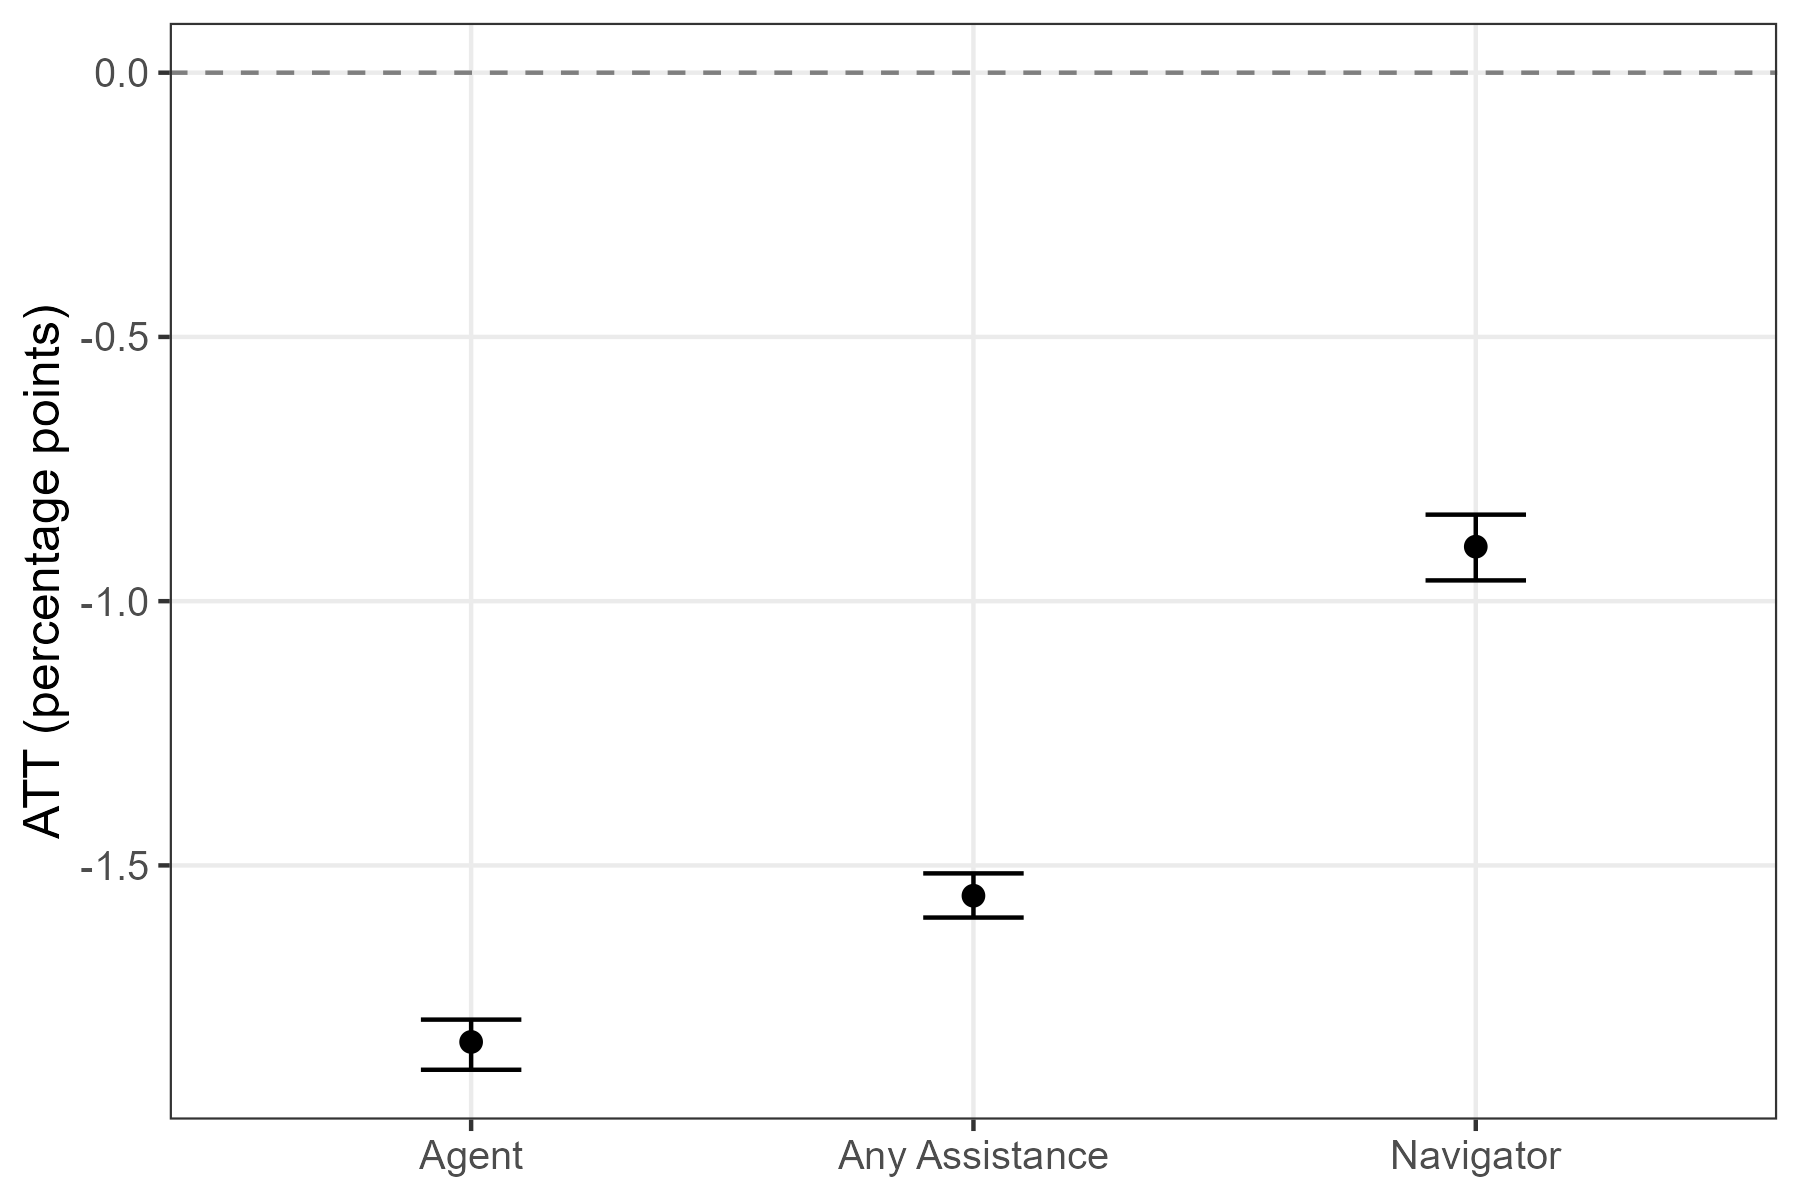
\includegraphics[width=\linewidth,height=0.72\textheight,keepaspectratio]{../results/figures/dom_choice.png}
    \column{0.40\textwidth}
      \onslide<2->{\textbf{\color{emoryBlue}Agent}\\[2pt]48\% reduction (1.8pp)\\[0.4cm]}
      \onslide<3->{\textbf{\color{emoryDark}Any assistance}\\[2pt]42\% reduction (1.6pp)\\[0.4cm]}
      \onslide<4->{\textbf{\color{emoryMid}Navigator}\\[2pt]25\% reduction (0.9pp)}
  \end{columns}
\end{frame}

% ── Structural Model ────────────────────────────────────────
\section{A Model of Choice and Pricing}
\sectionframe

\begin{frame}<1>[label=help-nest]{Households choose plans, possibly with help; insurers set premiums and commissions}
  \begin{center}
  \begin{tikzpicture}[
    node distance=0.9cm and 0.6cm,
    every node/.style={align=center,font=\small},
    box/.style={draw=emoryBlue,thick,rounded corners,fill=emoryLightBlue,
      minimum width=2.9cm,minimum height=1.0cm,text width=2.6cm},
    agentbox/.style={draw=emoryGold,thick,rounded corners,fill=emoryLight,
      minimum width=2.9cm,minimum height=1.0cm,text width=2.6cm},
    insbox/.style={draw=emoryBlue,thick,rounded corners,fill=emoryLightBlue,
      minimum width=7.2cm,minimum height=1.1cm,text width=6.8cm},
    arr/.style={-{Stealth[length=2.2mm]},thick,emoryMid},
    garr/.style={-{Stealth[length=2.2mm]},thick,emoryGold},
  ]
    \node[box] (hh) {Household};
    \node[box,below left=0.6cm and 1.6cm of hh] (unassist) {Unassisted};
    \node[box,below=1.0cm of hh] (nav) {Navigator};
    \node[agentbox,below right=0.6cm and 1.6cm of hh] (agent) {Agent};
    \node[insbox,below=0.9cm of nav] (insurer) {Insurer: sets premium $p$ and commission $y$};

    \draw[arr] (hh) -- (unassist);
    \draw[arr] (hh) -- (nav);
    \draw[garr] (hh) -- (agent);
    \draw[arr] (unassist) -- (insurer);
    \draw[arr] (nav) -- (insurer);
    \draw[garr] (agent) -- (insurer);
    \draw[arr,dashed,rounded corners=8pt] (insurer.east) -- ++(2.8,0) |- (hh.east)
      node[pos=0.75,above,font=\scriptsize,text=emoryMid,text width=4.2cm,align=center]
      {premiums and commissions feed back into household utility};
  \end{tikzpicture}
  \end{center}
  {\scriptsize\color{emoryMid} Insurers price against risk adjustment and subsidy rules; the commission channel (gold) is the mechanism we estimate.%
  \helpcard{help-nest}{{\bfseries How should the assistance channel enter demand?}\par\vspace{5pt}
  Plan choice is at the household's observed channel. Enrollment uses the average of the three channel inclusive values, weighted by first-stage channel probabilities.\par\vspace{5pt}
  A full three-level nest (plans within channel within enrollment) does not fit. The channel nesting parameter runs past the limit of 1 that utility maximization requires, and as it grows the model converges to our two-part version. Households do not appear to sort into channels on the plans each channel would lead to.\par\vspace{5pt}
  Is treating the channel as a circumstance rather than a choice reasonable, or is there a better way to model channel selection?}\par}
\end{frame}

\begin{frame}<1>[label=help-comm]{Commissions steer enrollment}
  A \$1 increase in monthly commission shifts agent-assisted enrollment as much as a \$1.47 reduction in net monthly premium.

  \vspace{0.3cm}
  In elasticity terms, a 1\% change in commissions moves agent-assisted demand roughly 0.22 as much as a 1\% change in premiums.

  \vspace{0.5cm}
  \begin{center}
  \begin{tikzpicture}
    \fill[emoryGold] (0,0) rectangle (3,0.9);
    \fill[emoryBlue] (3.7,0) rectangle (8.1,0.9);
    \node[below,font=\bfseries\small,text width=3.2cm,align=center] at (1.5,-0.05) {+\$1 commission};
    \node[below,font=\bfseries\small,text width=3.6cm,align=center] at (5.9,-0.05) {$-$\$1.47 net premium};
    \node[font=\scriptsize,color=emoryMid] at (4.05,1.25) {same shift in agent-assisted enrollment};
  \end{tikzpicture}
  \end{center}
  \helpcard{help-comm}{{\bfseries How do insurers set commissions?}\par\vspace{5pt}
  A commission pays the agent for enrollment and servicing the insurer would otherwise do in house. Each insurer sets its commission so the enrollment it steers is worth the marginal outlay, net of that saving and a carrier-level constant.\par\vspace{5pt}
  Solving for the level is fragile, since the implied rate is the difference of two numbers several times the observed commission. Curvature in the demand response to commissions stabilized it, and the carrier constants do much of the remaining fitting.\par\vspace{5pt}
  Is there a better model of commission setting, or a mechanism that could replace the carrier constants?}
\end{frame}

\begin{frame}{Why this matters}
  The model lets us separate three things that move together in the data:

  \vspace{0.4cm}
  \begin{center}
  \begin{tikzpicture}[
    box/.style={draw=emoryBlue,thick,rounded corners,fill=emoryLightBlue,
      minimum width=3.3cm,minimum height=2.5cm,text width=3.0cm,align=center,font=\small},
  ]
    \node<1->[box] (v) at (0,0) {{\Large\color{emoryBlue}+}\\[4pt]value assistance provides\\(better-matched plans)};
    \node<2->[box] (s) at (3.8,0) {{\Large\color{emoryGold}$-$}\\[4pt]steering commissions introduce\\(worse-matched plans)};
    \node<3->[box] (p) at (7.6,0) {{\Large\color{emoryMid}$\pm$}\\[4pt]premium pass-through of paying for commissions};
  \end{tikzpicture}
  \end{center}
\end{frame}

% ── Welfare and Counterfactuals ──────────────────────────────
\section{What Would Change Without Agents?}
\sectionframe

\begin{frame}{Counterfactual 1: withdraw decision assistance entirely}
  \begin{center}
    \statbox{6cm}{+6.1pp}{rise in the uninsured share}
  \end{center}

  \vspace{0.4cm}
  Welfare falls, driven mainly by lost coverage rather than worse plan matches among those who stay enrolled.
\end{frame}

\begin{frame}{Zeroing out commissions only helps once navigators replace what agents did}
  \only<1>{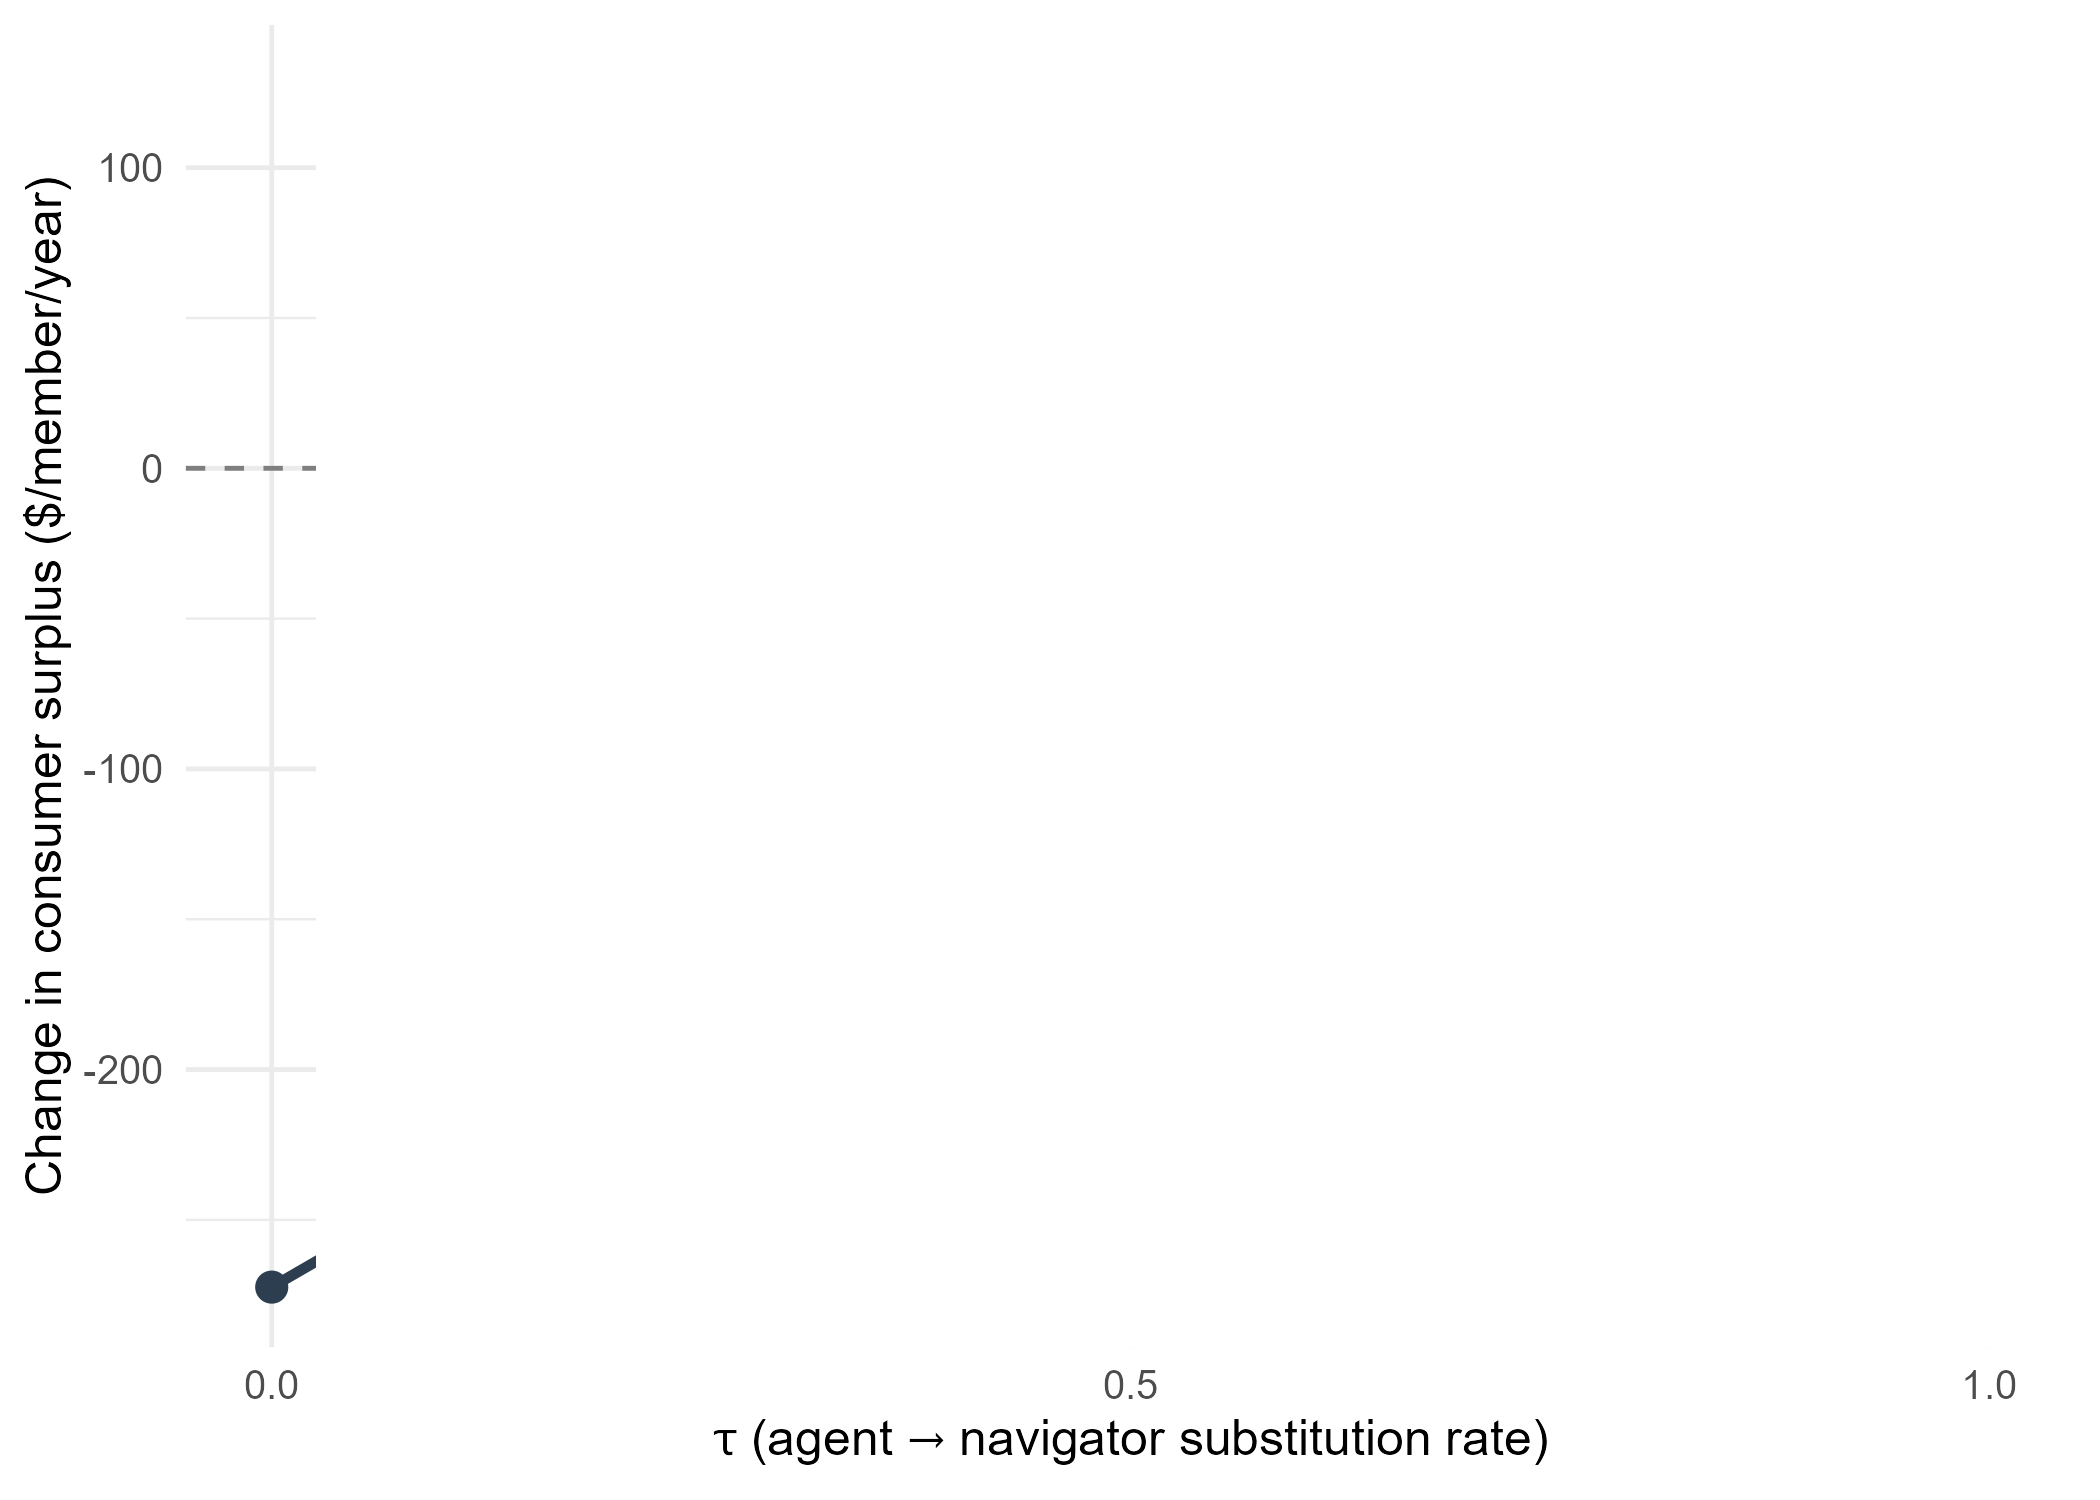
\includegraphics[width=\linewidth,height=0.54\textheight,keepaspectratio]{image/cf_gradient_reveal1.png}}%
  \only<2>{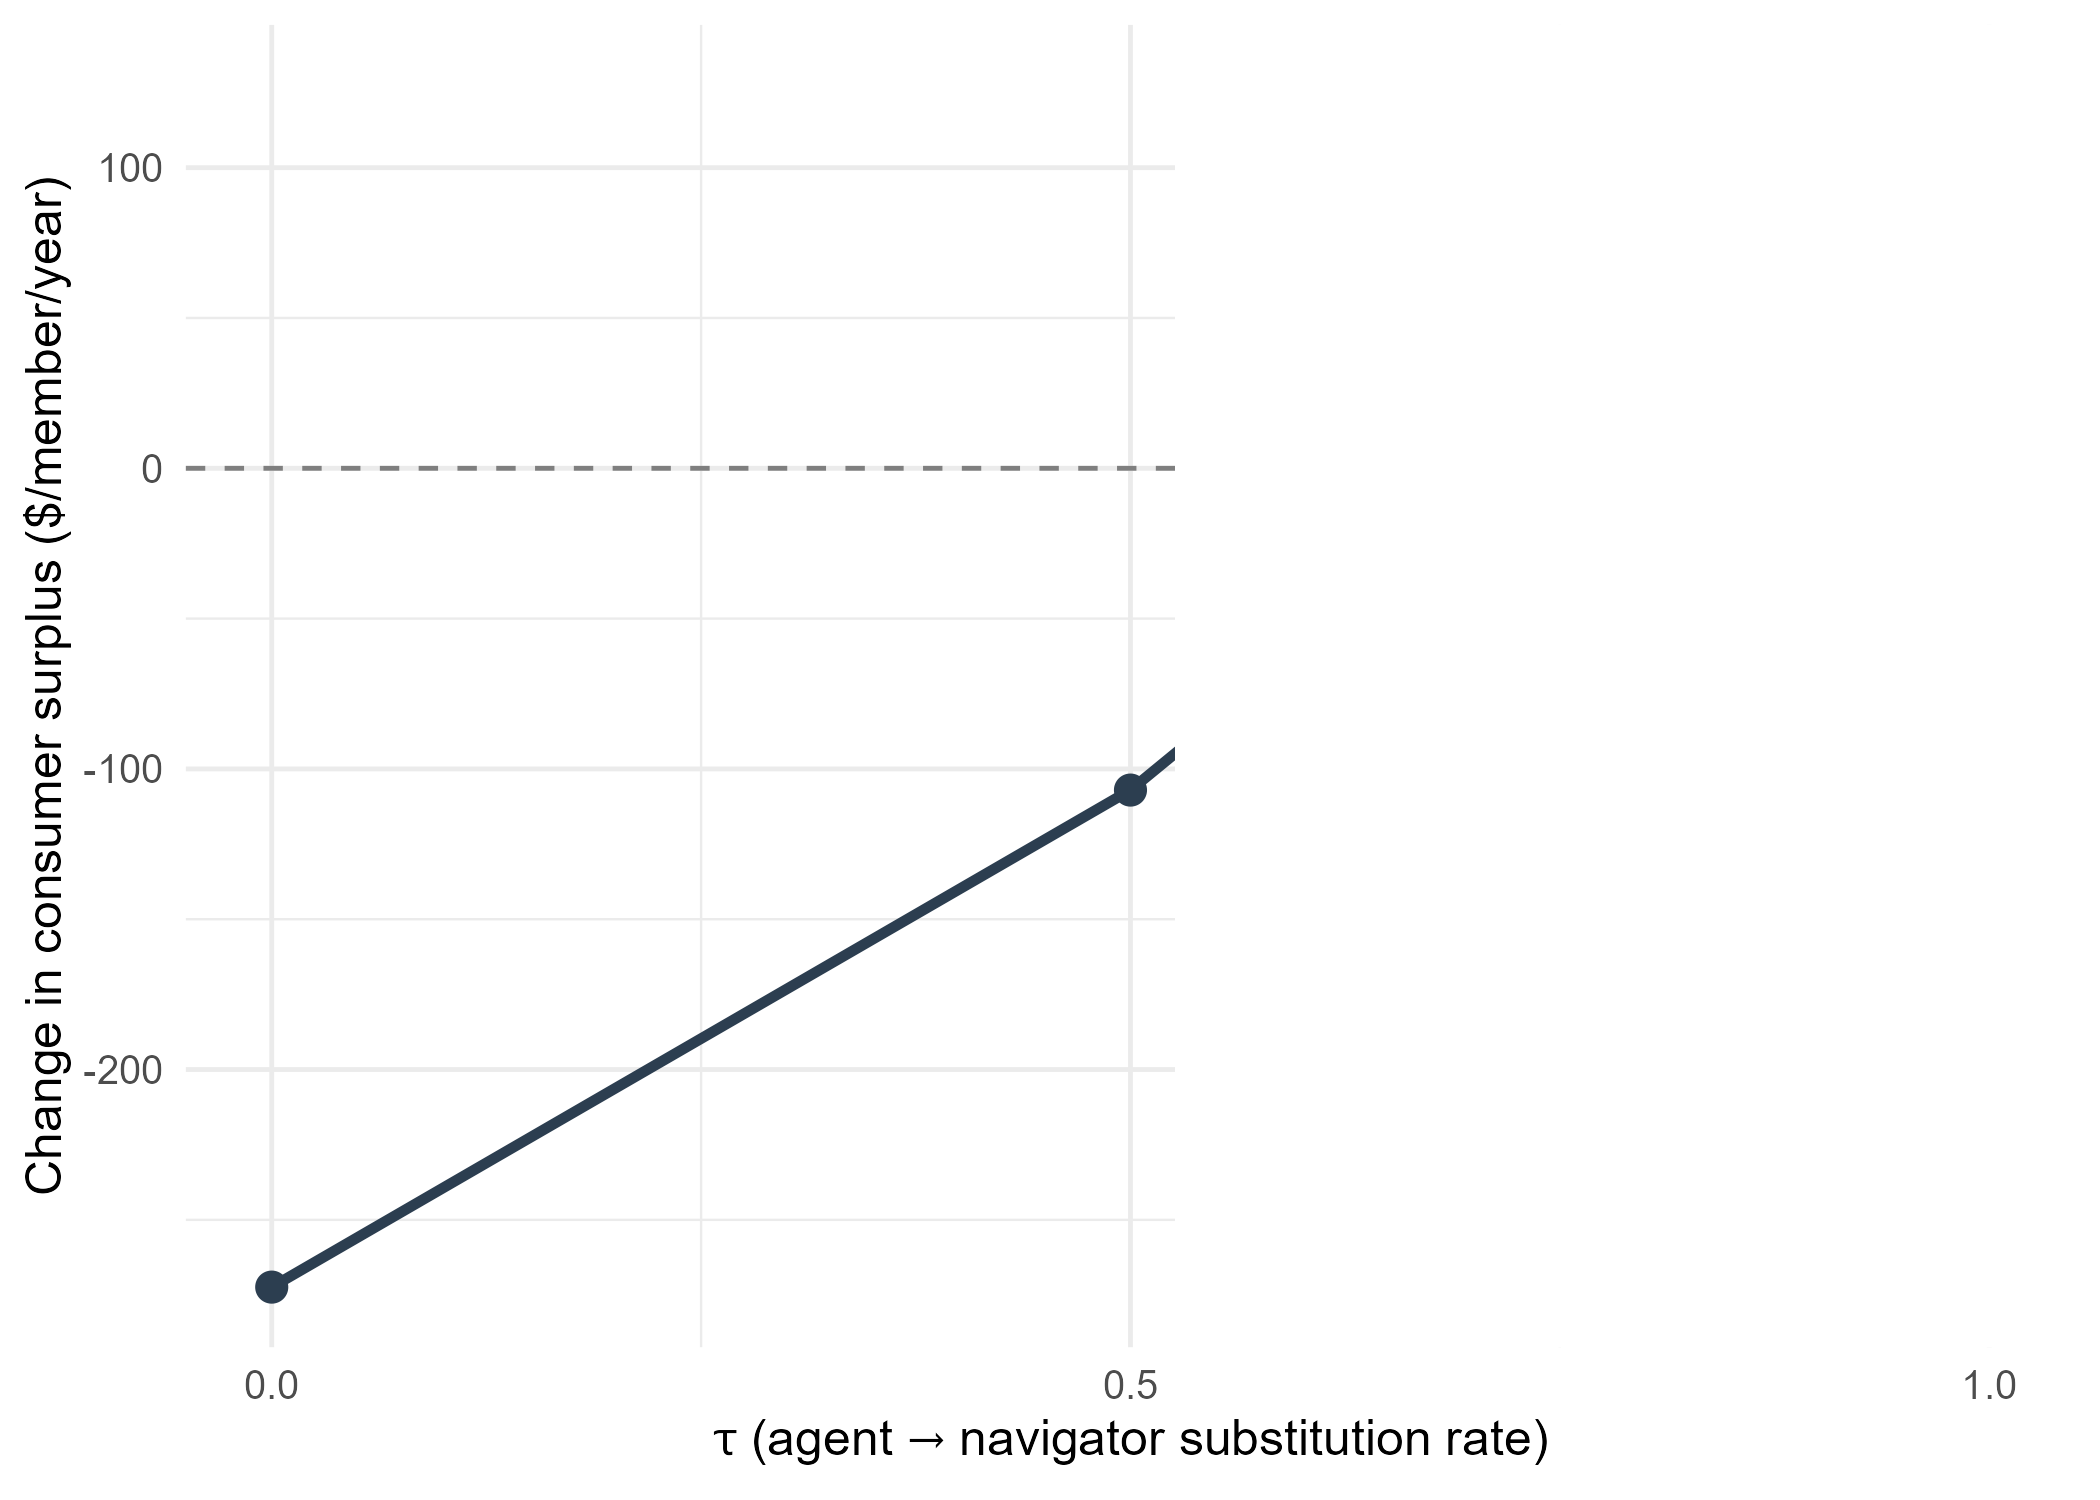
\includegraphics[width=\linewidth,height=0.54\textheight,keepaspectratio]{image/cf_gradient_reveal2.png}}%
  \only<3>{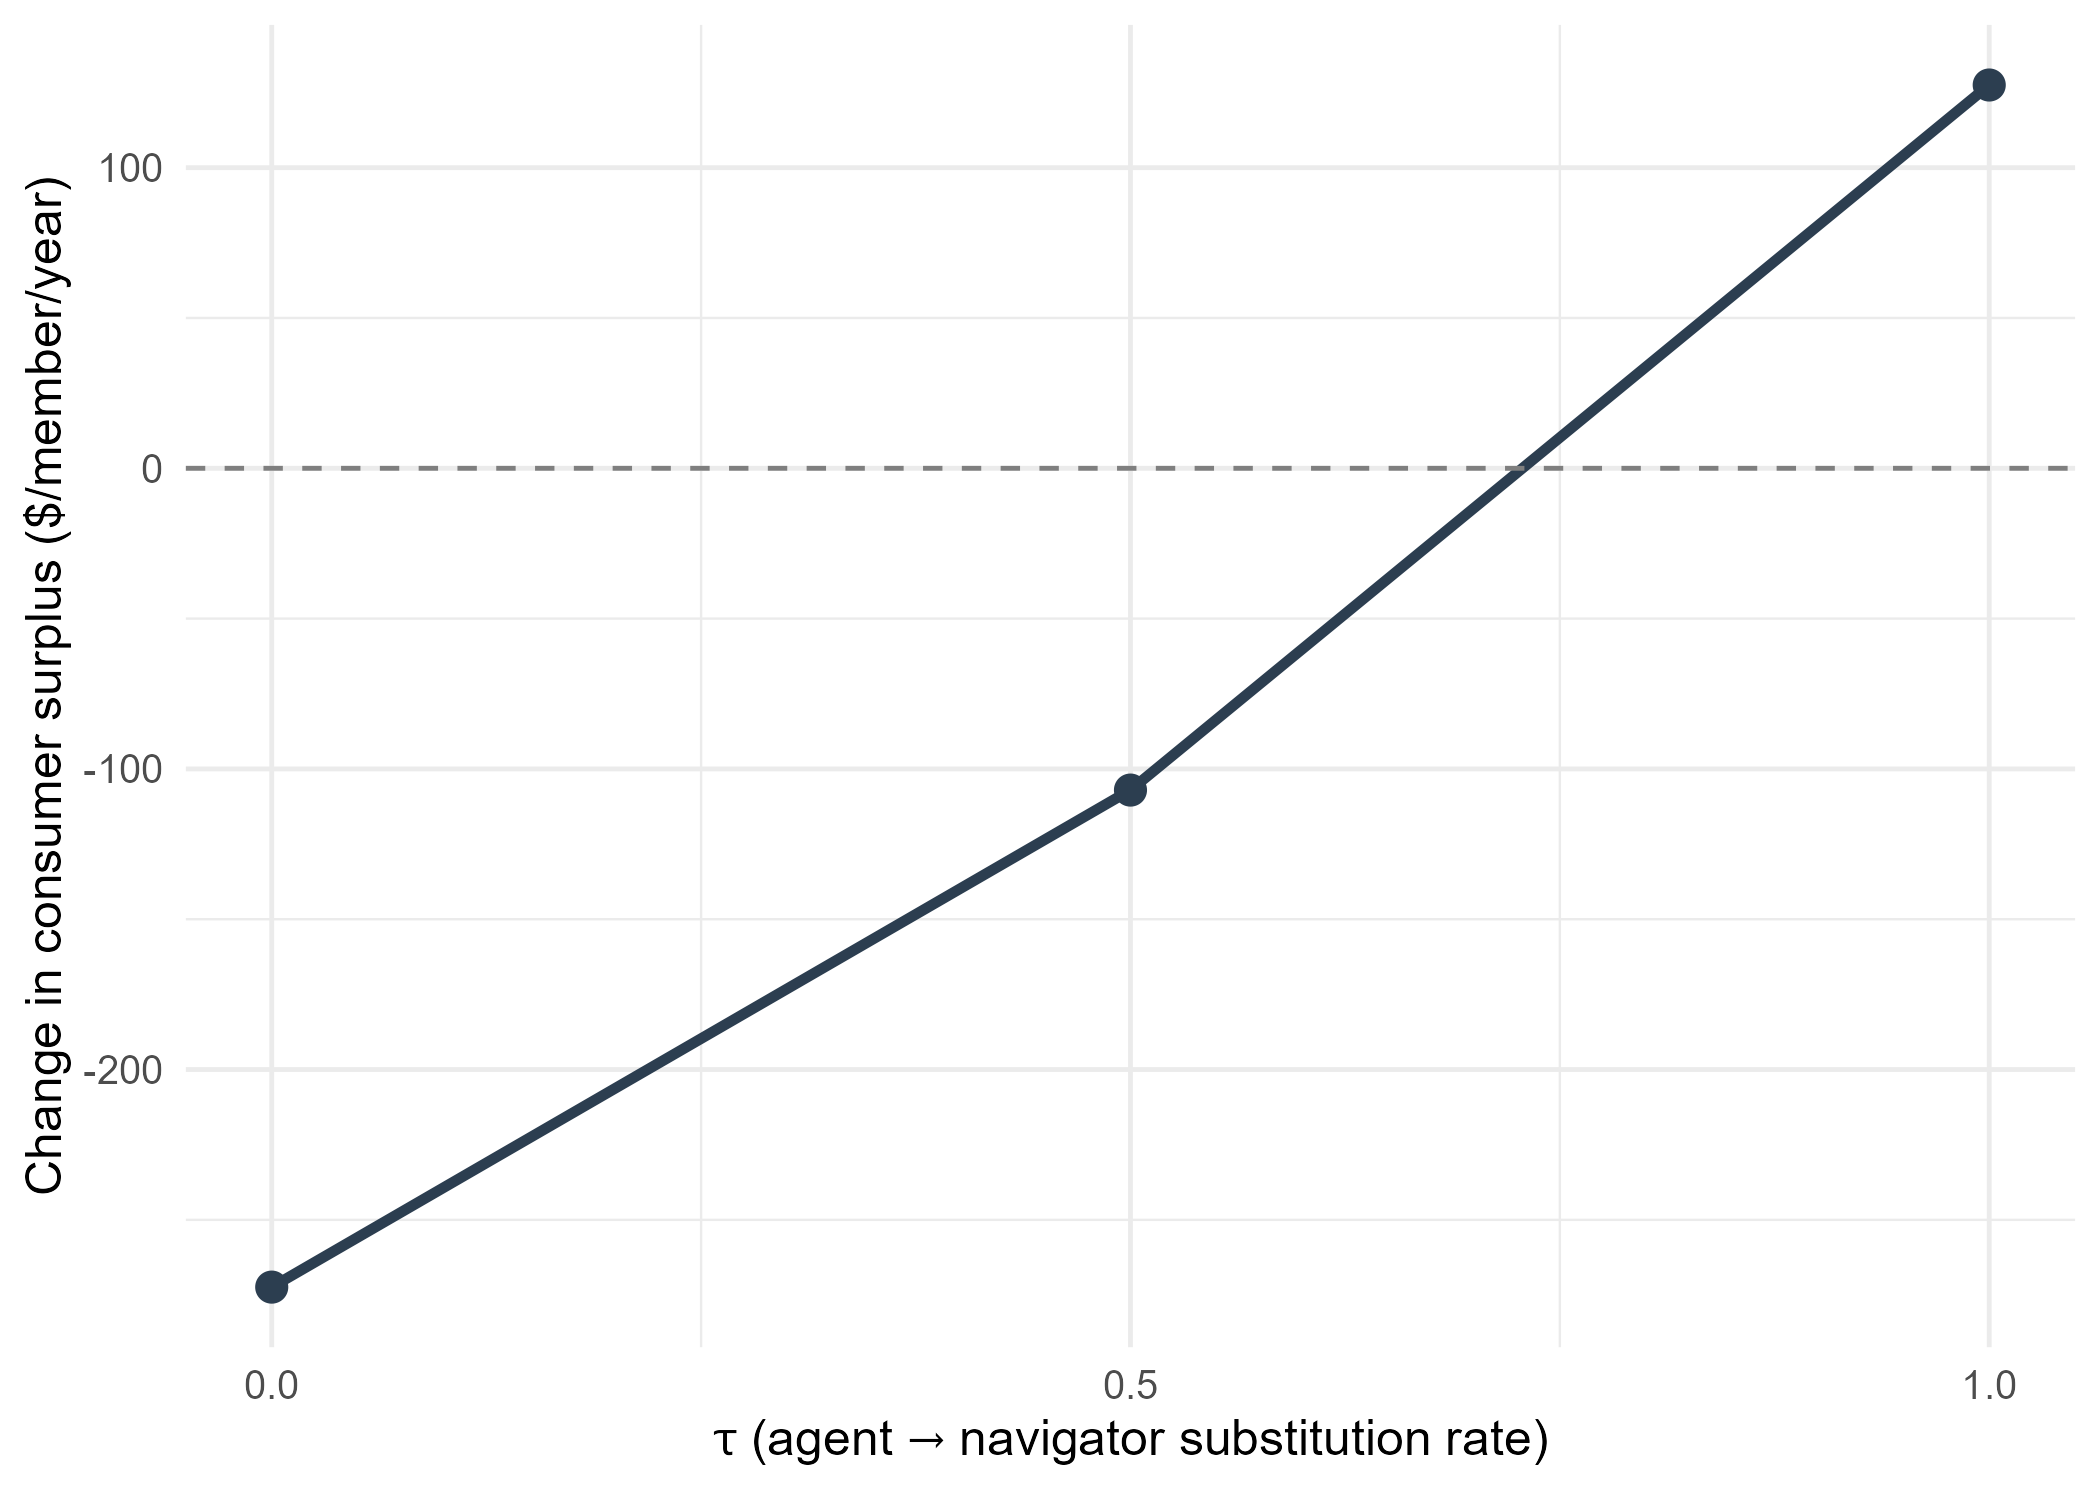
\includegraphics[width=\linewidth,height=0.54\textheight,keepaspectratio]{image/cf_gradient_reveal3.png}}%

  \vspace{0.1cm}
  \small
  \onslide<1>{\centering\textcolor{emoryMid}{$\tau=0$: formerly agent-assisted households become unassisted. Welfare falls.}\par}
  \onslide<2>{\centering\textcolor{emoryMid}{$\tau=0.5$: half shift to navigators instead. Still negative, but less so.}\par}
  \onslide<3>{\centering\textcolor{emoryMid}{$\tau=1$: all shift to navigators. Premium savings now dominate, and welfare turns positive.}\par}
\end{frame}

\begin{frame}{Counterfactual 2: reshape the commission schedule, keep assistance}
\figureslide{%
  \small
  Welfare changes by less than \$70 per member per year.

  \vspace{0.2cm}
  Coverage barely moves. Commission \emph{design} is a second-order lever relative to whether assistance exists at all.

  \vspace{0.2cm}
  {\scriptsize\color{emoryMid} Premiums also move only modestly across these alternative commission schedules.}
}{../results/figures/cf_premium_change.png}
\end{frame}

\begin{frame}{Counterfactual 3: replace private agents with public navigators}
  \begin{center}
    \onslide<1->{\statbox{4cm}{$-$\$54}{premiums, per member per year}}%
    \onslide<2->{\statbox{4cm}{$-$0.2pp}{uninsured share}}%
    \onslide<3->{\statbox{4cm}{+\$30}{welfare, per member per year}}
  \end{center}

  \vspace{0.5cm}
  \onslide<4->{Premiums fall because insurers no longer pass commission costs through to all enrollees, and navigators keep households insured.}
\end{frame}

\begin{frame}{Counterfactual 4: shifting households between navigators and agents moves welfare little}
  \begin{columns}[t,onlytextwidth]
    \column{0.47\textwidth}
      {\bfseries\color{emoryBlue} Navigator defunding}\\[2pt]
      {\small Half of navigator households shift to agents; commissions re-solve.}
      \begin{itemize}
        \item Premiums +\$9
        \item Uninsured share +0.1pp
        \item Welfare $-$\$12 per member per year
      \end{itemize}
    \column{0.47\textwidth}
      \onslide<2->{%
      {\bfseries\color{emoryBlue} Navigator expansion}\\[2pt]
      {\small Half of agent households shift to navigators; the rest keep agents, and commissions re-solve.}
      \begin{itemize}
        \item Premiums $-$\$21
        \item Uninsured share $-$0.1pp
        \item Welfare +\$12 per member per year
      \end{itemize}}
  \end{columns}
\end{frame}

% ── Conclusion ───────────────────────────────────────────────
\section{Conclusion}
\sectionframe

\begin{frame}{Decision assistance is worth having; who pays for it matters less than whether it exists}
  \onslide<1->{\textbf{\color{emoryBlue}Assistance helps.} Assistance improves plan choice; losing it costs coverage, not just match quality.}

  \vspace{0.35cm}
  \onslide<2->{\textbf{\color{emoryGold}Steering is large; its welfare cost is small.} Commissions move agent-assisted enrollment substantially, but cost households little relative to the value of assistance itself.}

  \vspace{0.35cm}
  \onslide<3->{\textbf{\color{emoryMid}Policy is live.} Federal navigator funding has been cut, restored, and cut again; MA has tried to cap agent commissions on steering grounds.}
\end{frame}

% Bibliography
% \bibliographystyle{aer}
% \bibliography{BibTeX_Library}

% Closing
\closingframe{Ian McCarthy}{%
  Department of Economics, Emory University\\[0.15cm]
  \href{mailto:ian.mccarthy@emory.edu}{ian.mccarthy@emory.edu}\\[0.1cm]
  \href{https://ianmccarthyecon.com}{ianmccarthyecon.com}%
}

%% ── Appendix ─────────────────────────────────────────────────
\appendix
\section{Appendix}

\begin{frame}{Dropping plan-based enrollers makes the steering estimate slightly stronger, not weaker}
  Plan-based enrollers are a single-insurer channel (1.3\% of the structural sample) whose influence works through a restricted menu, not a commission.

  \vspace{0.3cm}
  Re-estimating the demand model without them leaves price, actuarial value, and nesting parameters essentially unchanged; the commission-steering coefficients move from 0.027/$-0.066$ to 0.030/$-0.070$.

  \vspace{0.3cm}
  A single-insurer channel is not what generates the estimated steering.
\end{frame}

\begin{frame}{A menu restriction and a commission in utility predict the same choices, but not the same counterfactuals}
  We represent agent steering as a commission term in utility rather than a restricted menu. A gatekeeper simulation checks this: generate choices from a menu that is restricted by commission (no commission in utility), then fit our model to them.

  \vspace{0.3cm}
  The fitted model reproduces the gatekeeper's agent shares to within 1.1--1.7 percentage points (correlation above 0.997), even when the menu restriction is also selected on agent or household characteristics.

  \vspace{0.3cm}
  The two representations are observationally equivalent for demand, but a fixed menu restriction cannot respond to a change in commissions. The counterfactuals therefore need the commission margin, not just the demand fit.
\end{frame}

\begin{frame}{The commission first-order condition sets marginal steering benefit against marginal payout, unit by unit}
  Demand is a two-part nested logit: plan choice uses the household's realized assistance channel, enrollment uses the expected inclusive value across the three channel states, so commissions can move coverage as well as plan choice.

  \vspace{0.3cm}
  The premium FOC is a standard markup condition, augmented with the risk-adjustment transfer and the commission outlay.

  \vspace{0.3cm}
  The commission FOC holds one condition per commission-setting unit (insurer, or insurer-network where the filed schedule sets separate rates). It sets the ratio of marginal steering benefit, the added profit from commission-induced enrollment plus the risk-adjustment feedback, to marginal outlay equal to $(1-\beta_f) + \delta_f$, where $\beta_f$ is the administrative saving per commission dollar and $\delta_f$ is a carrier-level constant estimated jointly with the cost parameters.
\end{frame}

% Help! cards (reached only from their buttons)
\againframe<2>{help-nest}
\againframe<2>{help-comm}

\end{document}
